\documentclass[11pt,a4paper]{article}

\usepackage[utf8]{inputenc}
\usepackage[T1]{fontenc}
\usepackage[brazil]{babel}
\usepackage{lmodern}
\usepackage{microtype}
\usepackage{geometry}
\usepackage{graphicx}
\usepackage{booktabs}
\usepackage{tabularx}
\usepackage{array}
\usepackage{float}
\usepackage{caption}
\usepackage{subcaption}
\usepackage{enumitem}
\usepackage{xcolor}
\usepackage{hyperref}
\usepackage{fancyhdr}
\usepackage{setspace}

\geometry{top=2.5cm,bottom=2.5cm,left=2.7cm,right=2.7cm}
\setstretch{1.15}
\setlength{\parindent}{1.25cm}
\setlength{\parskip}{0.15cm}
\setlist{noitemsep,topsep=3pt}
\captionsetup{font=small,labelfont=bf}
\definecolor{ecoscan}{HTML}{1B5E20}
\definecolor{linkblue}{HTML}{0D47A1}
\hypersetup{colorlinks=true,linkcolor=linkblue,citecolor=ecoscan,urlcolor=linkblue,pdftitle={EcoScan Classificacao de Residuos por Imagem},pdfauthor={Leonardo Bonatto Fernandes e Gustavo Toledo Denig}}

\pagestyle{fancy}
\fancyhf{}
\fancyhead[L]{\small EcoScan}
\fancyhead[R]{\small Mineração de Dados}
\fancyfoot[C]{\thepage}
\renewcommand{\headrulewidth}{0.3pt}

\title{\textbf{EcoScan: classificação de resíduos por imagem com Mineração de Dados}}
\author{Leonardo Bonatto Fernandes \\ Gustavo Toledo Denig}
\date{Novembro de 2026}

\begin{document}
\maketitle

\begin{abstract}
A separação incorreta de resíduos reduz o aproveitamento de materiais recicláveis e aumenta o esforço necessário para a triagem. Este trabalho apresenta o EcoScan, um projeto de Mineração de Dados voltado à classificação de resíduos em seis categorias: metal, papel, papelão, plástico, rejeito e vidro. Foram integradas as bases públicas TrashNet e RealWaste, totalizando 6.114 imagens válidas. O processo foi organizado segundo o CRISP-DM e incluiu validação dos arquivos, padronização de rótulos, análise exploratória, tratamento do desbalanceamento, transformação das imagens em atributos numéricos e comparação de três modelos do Scikit-Learn. As características visuais foram representadas por Histogram of Oriented Gradients (HOG) e histogramas de cor no espaço HSV. Entre os algoritmos avaliados, a máquina de vetores de suporte com kernel RBF apresentou o melhor resultado, com acurácia de 66,88\% e F1 macro de 65,06\%. Um experimento adicional mostrou que o F1 macro caiu de 67,49\% em imagens controladas da TrashNet para 17,21\% em imagens reais da RealWaste. O resultado evidencia que a diversidade e a representatividade dos dados são determinantes para a aplicação prática do modelo. O protótipo inclui uma API em FastAPI para consulta do classificador treinado.
\end{abstract}

\noindent\textbf{Palavras-chave:} mineração de dados; classificação de imagens; resíduos recicláveis; aprendizado de máquina; CRISP-DM.

\section{Introdução}

A separação de resíduos é uma etapa importante para a reciclagem, pois materiais descartados na categoria errada podem ser contaminados e perder seu potencial de reaproveitamento. Em empresas, condomínios, instituições de ensino e centrais de triagem, a identificação do material depende frequentemente de avaliação humana. Esse processo pode ser repetitivo e sujeito a divergências, sobretudo quando os objetos estão deformados, sujos ou misturados.

O EcoScan foi proposto como uma ferramenta de apoio à classificação inicial de resíduos por imagem. A pergunta principal da pesquisa é: \textit{um modelo treinado com imagens de resíduos em ambiente controlado mantém seu desempenho quando aplicado a imagens capturadas em condições reais?} A pergunta incorpora uma preocupação central levantada na etapa inicial do projeto: um resultado satisfatório em uma base organizada não garante funcionamento no ambiente de uso.

O objetivo geral foi desenvolver e avaliar um fluxo completo de Mineração de Dados capaz de classificar imagens de resíduos. Os objetivos específicos foram: integrar duas bases públicas, analisar a qualidade e o balanceamento dos dados, transformar imagens em variáveis numéricas, comparar modelos do Scikit-Learn, avaliar a mudança de domínio entre imagens controladas e reais e disponibilizar o melhor modelo por uma API experimental.

Foram consideradas as seguintes hipóteses: (i) um modelo supervisionado alcança desempenho superior a uma classificação aleatória; (ii) classes visualmente próximas apresentam mais confusões; (iii) quantidade e diversidade de imagens influenciam o desempenho; e (iv) um modelo treinado apenas em imagens controladas perde desempenho quando aplicado a imagens reais.

\section{Fundamentação teórica}

\subsection{Mineração de Dados e CRISP-DM}

Mineração de Dados é o processo de identificação de padrões úteis em conjuntos de dados por meio de técnicas estatísticas e computacionais. Neste trabalho foi adotado o CRISP-DM, que organiza o projeto em seis etapas: compreensão do negócio, compreensão dos dados, preparação dos dados, modelagem, avaliação e implantação \cite{wirth2000crisp}. A metodologia foi escolhida por permitir a revisão de decisões conforme novos resultados são encontrados.

\subsection{Representação das imagens}

Os modelos tradicionais de aprendizado de máquina não recebem diretamente o significado visual de uma fotografia. Por isso, cada imagem foi convertida em um vetor de atributos. O HOG descreve padrões de bordas e formas por meio da distribuição das orientações dos gradientes \cite{dalal2005hog}. Para complementar a textura, foram calculados histogramas dos canais de matiz, saturação e brilho no espaço HSV. A combinação representa forma e cor sem utilizar uma rede neural profunda.

\subsection{Modelos avaliados}

Foram avaliados três algoritmos implementados pelo Scikit-Learn \cite{pedregosa2011scikit}: Regressão Logística, Random Forest e máquina de vetores de suporte (SVM) com kernel RBF. A Regressão Logística foi utilizada como referência linear; o Random Forest representa relações não lineares por um conjunto de árvores; e a SVM RBF permite construir fronteiras não lineares em espaços de muitas dimensões.

\section{Metodologia}

\subsection{Compreensão do problema}

O problema de negócio consiste em apoiar a triagem inicial de resíduos e produzir informações que possam ser usadas em ações de conscientização e gestão. O modelo não substitui a análise humana em situações ambíguas. Sua função é oferecer uma sugestão de classe e uma pontuação de confiança para apoiar a decisão.

\subsection{Bases de dados}

A RealWaste foi adotada como base principal por conter imagens coletadas em um ambiente real de aterro, no Whyte's Gully Waste and Resource Recovery Centre, em Wollongong, Austrália \cite{single2023realwaste}. A base original possui 4.752 imagens distribuídas em nove classes. Foram utilizadas as seis classes compatíveis com a TrashNet, resultando em 3.587 imagens.

A TrashNet foi utilizada como base complementar. Ela contém 2.527 imagens fotografadas predominantemente sobre fundo branco e distribuídas entre seis classes \cite{thung2016trashnet}. As categorias das duas fontes foram padronizadas para metal, papel, papelão, plástico, rejeito e vidro. A Tabela~\ref{tab:classes} apresenta a distribuição utilizada.

\begin{table}[H]
\centering
\caption{Quantidade de imagens por classe e por fonte}
\label{tab:classes}
\begin{tabular}{lrrr}
\toprule
\textbf{Classe} & \textbf{TrashNet} & \textbf{RealWaste} & \textbf{Total} \\
\midrule
Metal & 410 & 790 & 1.200 \\
Papel & 594 & 500 & 1.094 \\
Papelão & 403 & 461 & 864 \\
Plástico & 482 & 921 & 1.403 \\
Rejeito & 137 & 495 & 632 \\
Vidro & 501 & 420 & 921 \\
\midrule
\textbf{Total} & \textbf{2.527} & \textbf{3.587} & \textbf{6.114} \\
\bottomrule
\end{tabular}
\end{table}

\begin{figure}[H]
\centering
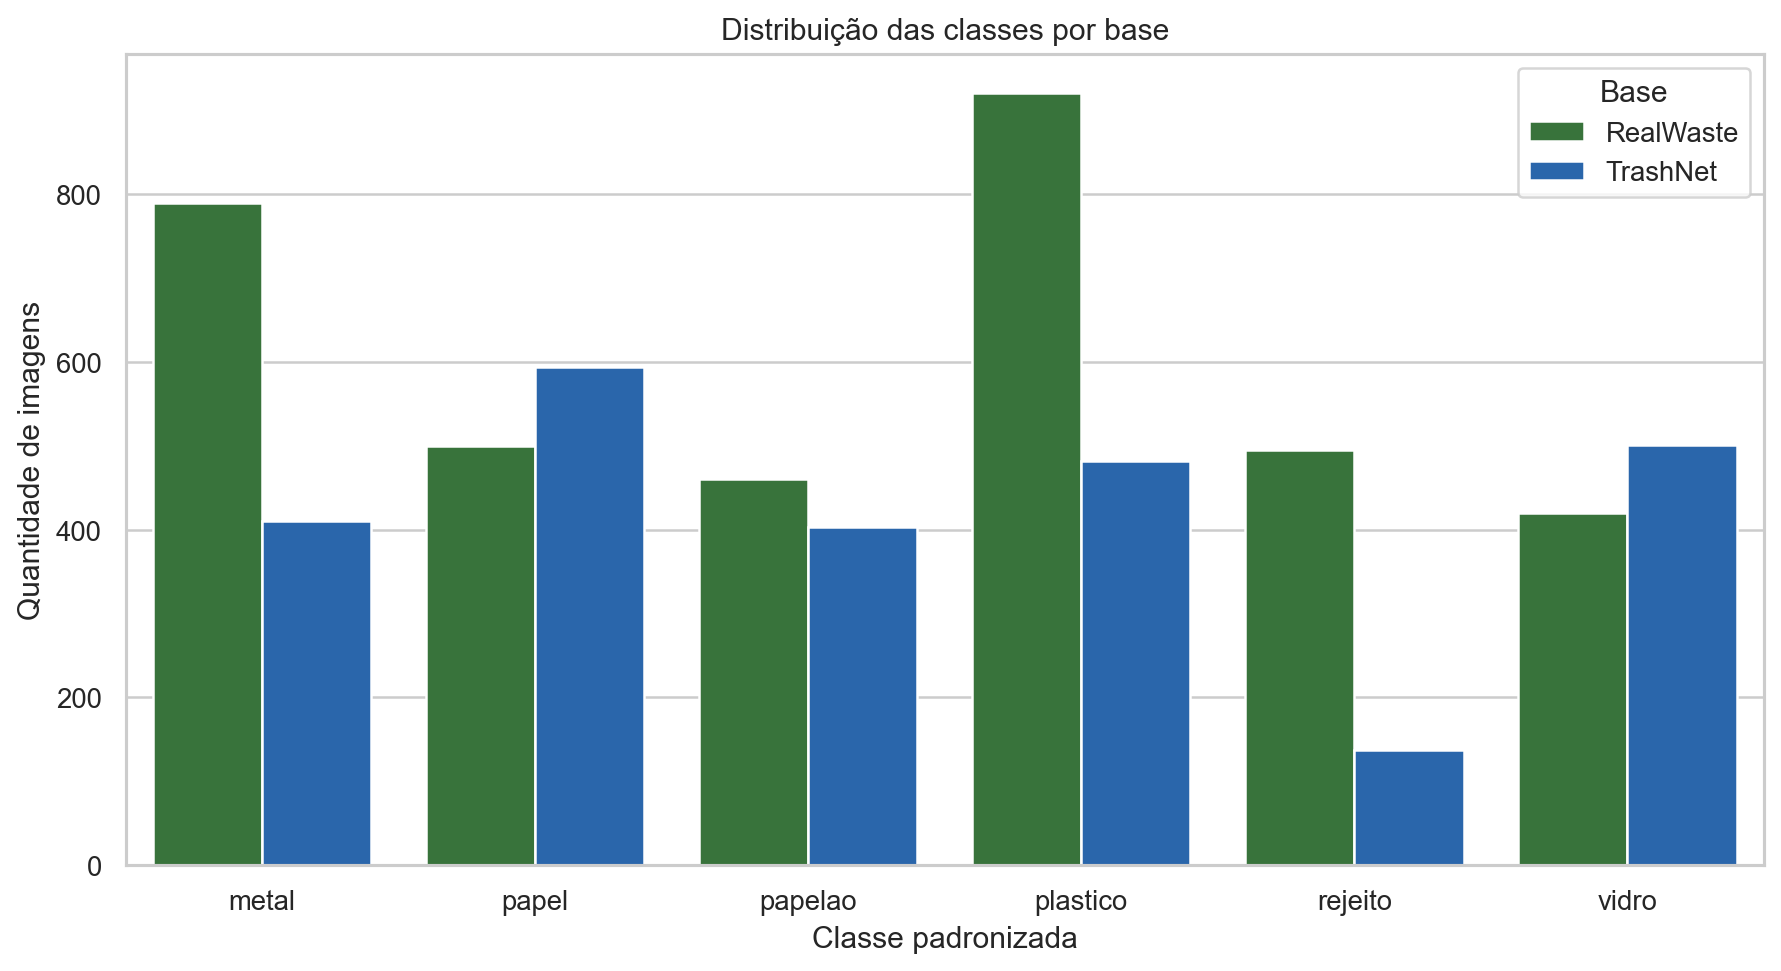
\includegraphics[width=0.88\textwidth]{images/01_distribuicao_classes.png}
\caption{Distribuição das classes nas bases TrashNet e RealWaste.}
\label{fig:distribuicao}
\end{figure}

\subsection{Limpeza, filtragem e transformação}

O processamento foi realizado em Python com NumPy \cite{harris2020numpy} e Pandas \cite{mckinney2010pandas}. Primeiro, os arquivos compactados foram extraídos e todas as imagens com extensões aceitas foram catalogadas. Cada arquivo foi aberto com a biblioteca Pillow para verificar sua integridade, dimensões e modo de cor. Não foram encontrados arquivos corrompidos nas seis classes selecionadas, portanto as 6.114 imagens puderam ser mantidas.

Os rótulos em inglês e com grafias diferentes foram transformados em seis nomes padronizados em português. As classes exclusivas da RealWaste, como resíduos orgânicos, vegetação e tecidos, foram filtradas para permitir a comparação direta entre as bases. As imagens foram convertidas para RGB, corrigidas conforme a orientação EXIF e redimensionadas para 64 por 64 pixels. Os valores dos canais foram normalizados para o intervalo de zero a um com NumPy.

Para cada imagem, foram extraídos 1.812 atributos: descritores HOG de textura e 16 intervalos de histograma para cada canal HSV. O manifesto final foi salvo em CSV e a matriz de características foi armazenada com Joblib para tornar os experimentos reproduzíveis.

\subsection{Análise exploratória e desbalanceamento}

Os gráficos foram produzidos com Matplotlib \cite{hunter2007matplotlib} e Seaborn \cite{waskom2021seaborn}. A Figura~\ref{fig:amostras} mostra que a TrashNet apresenta objetos isolados e fundos mais uniformes, enquanto a RealWaste contém sujeira, deformações, sobreposição e fundos complexos.

\begin{figure}[H]
\centering
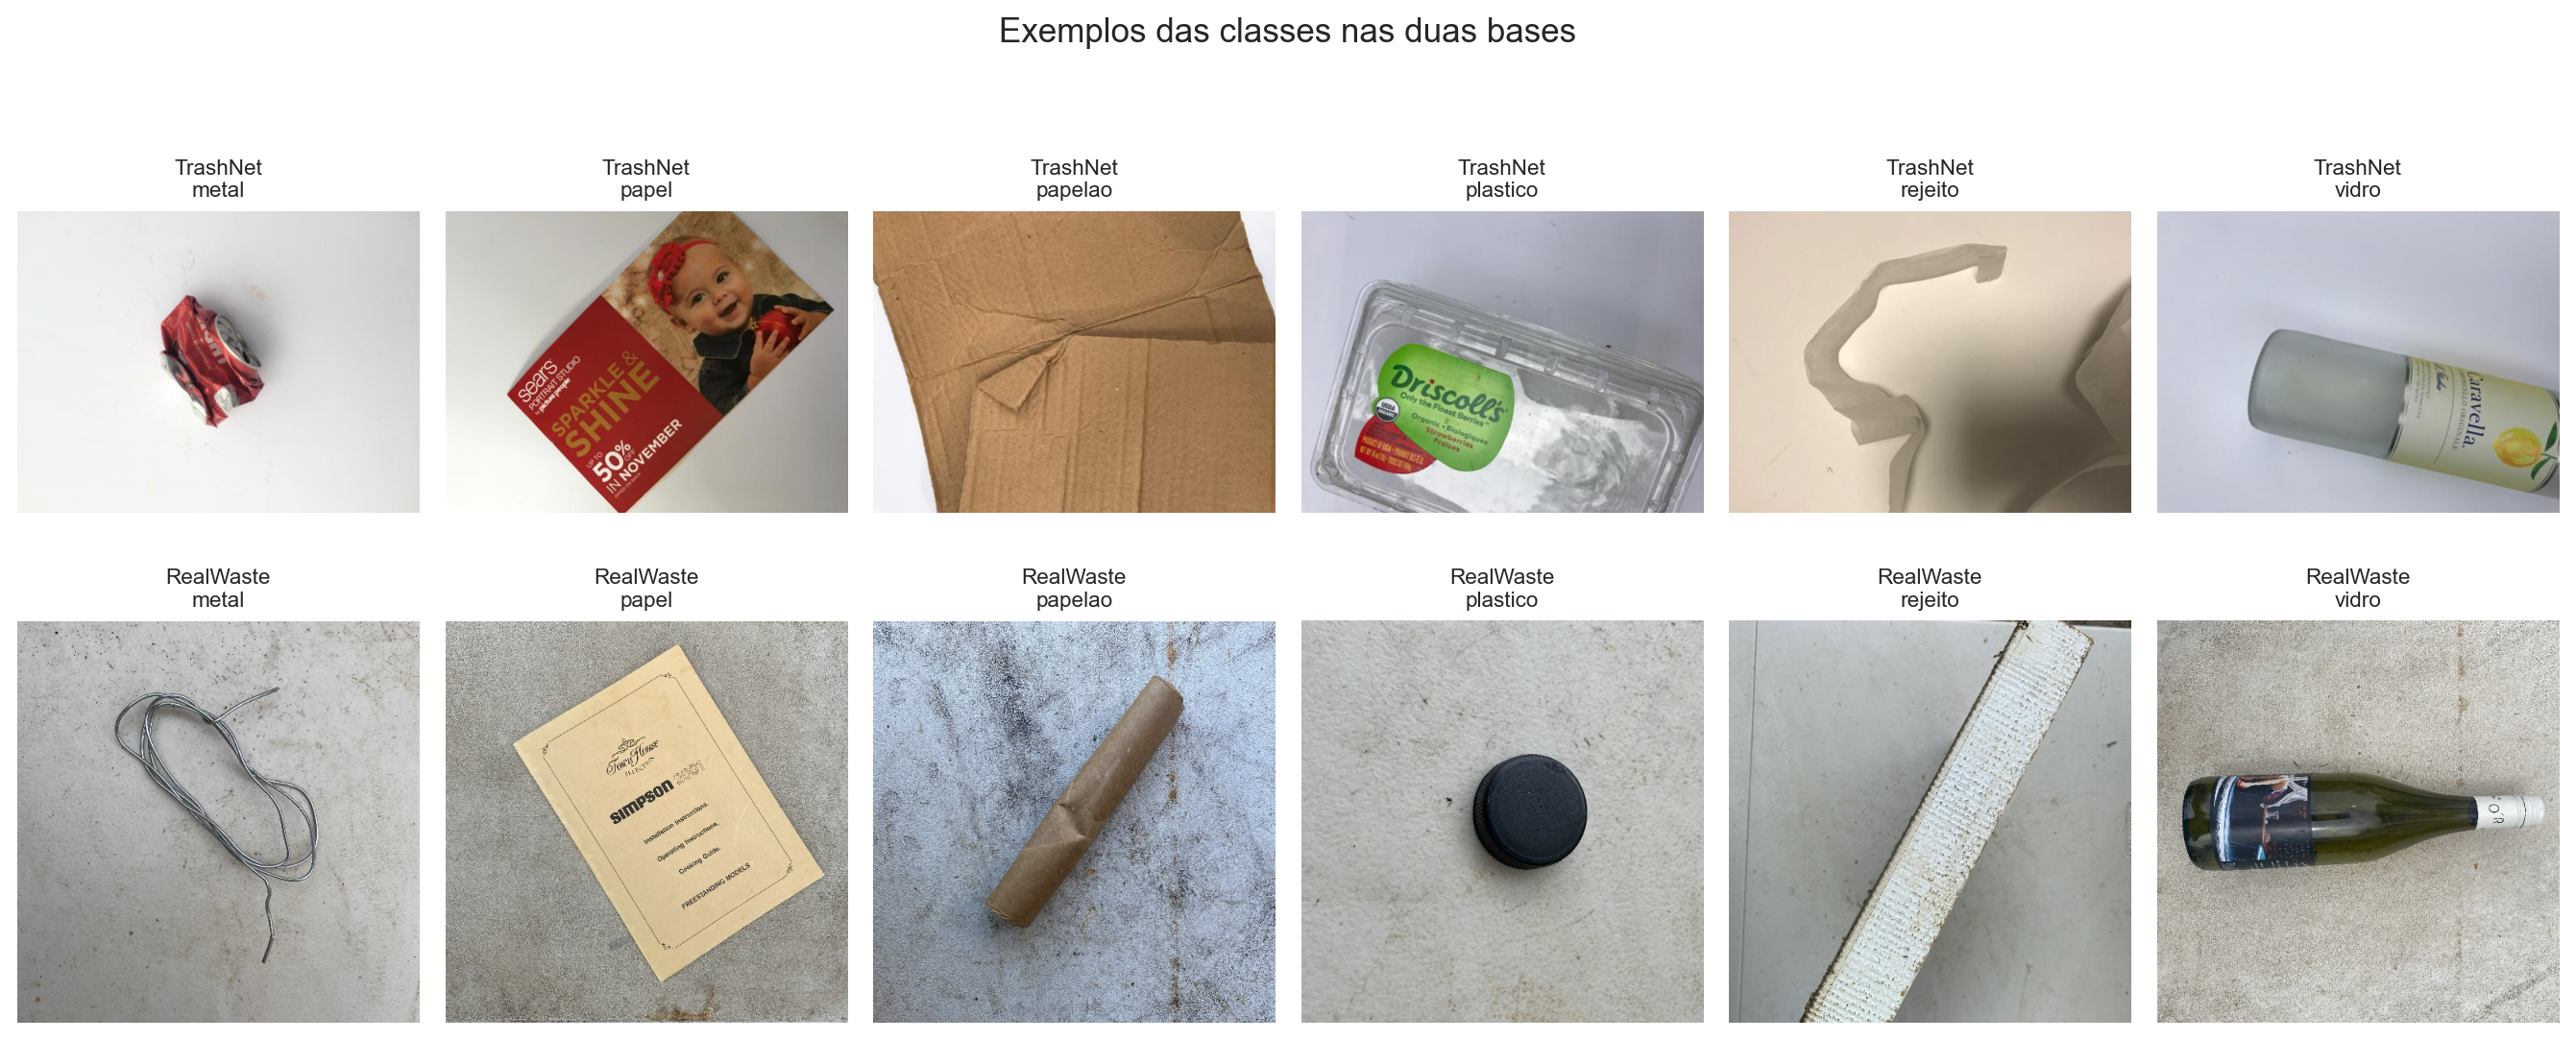
\includegraphics[width=\textwidth]{images/04_amostras_bases.png}
\caption{Exemplos das seis classes em cada base.}
\label{fig:amostras}
\end{figure}

O conjunto combinado é desbalanceado. Plástico possui 1.403 imagens, enquanto rejeito possui 632. Não foi utilizada duplicação simples das observações, pois isso poderia aumentar o sobreajuste. O tratamento ocorreu por pesos de classe inversamente relacionados à frequência, disponíveis nos três modelos, e por divisão estratificada, preservando a proporção das classes nos conjuntos de treino e teste.

\begin{figure}[H]
\centering
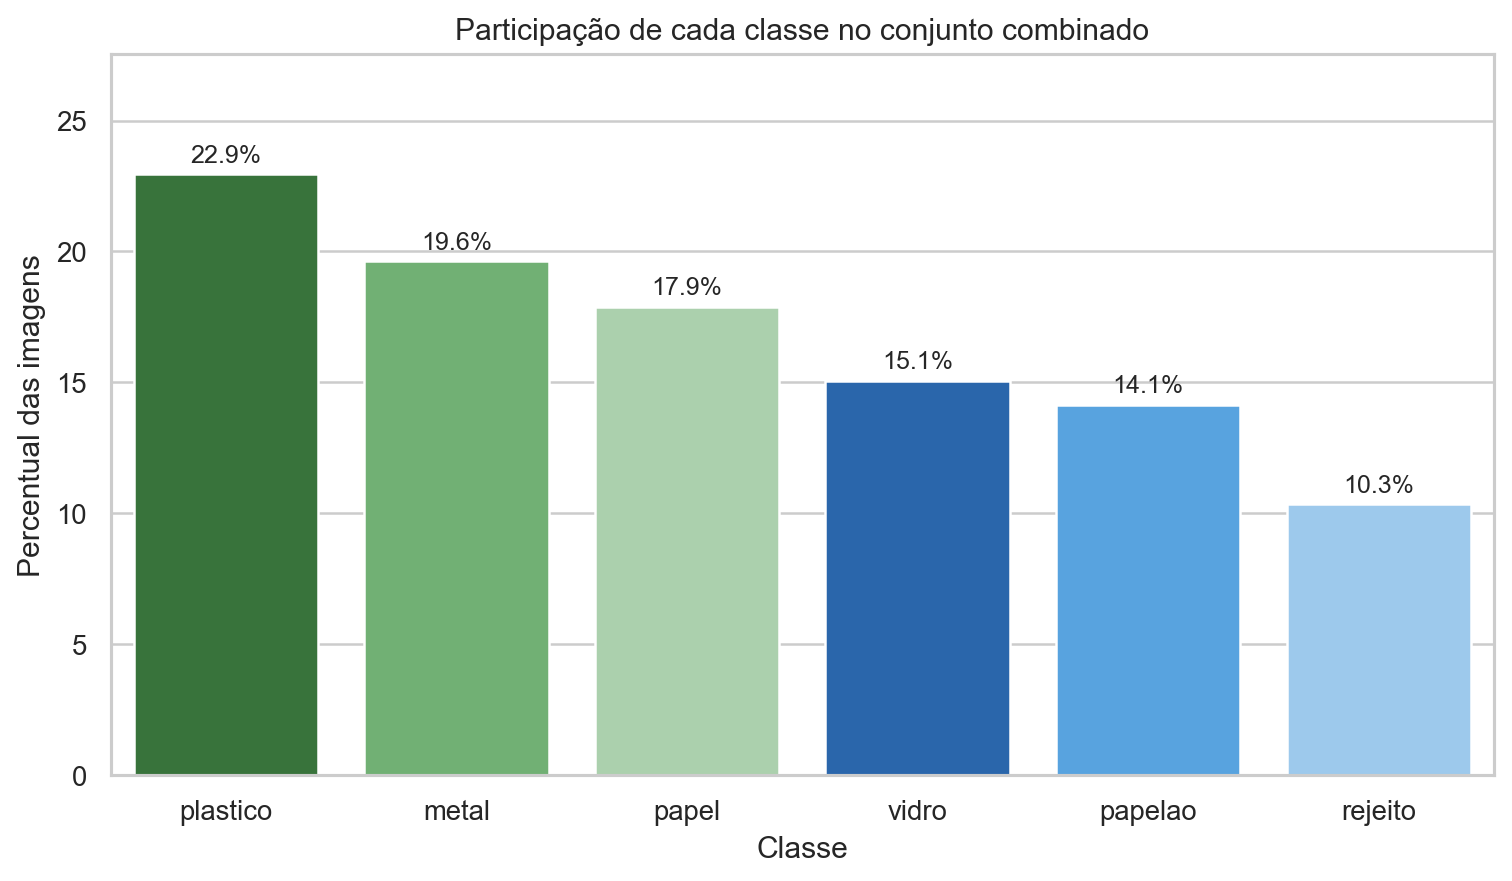
\includegraphics[width=0.84\textwidth]{images/02_balanceamento_percentual.png}
\caption{Participação percentual das classes no conjunto combinado.}
\label{fig:balanceamento}
\end{figure}

\subsection{Treinamento e avaliação}

O conjunto combinado foi dividido de forma estratificada em 80\% para treinamento e 20\% para teste, com semente aleatória 42. Foram utilizadas 4.891 imagens no treinamento e 1.223 no teste. A padronização dos atributos foi aplicada à Regressão Logística e à SVM dentro de um \textit{Pipeline}, evitando que informações do teste influenciassem o ajuste.

A Regressão Logística utilizou regularização com $C=1$ e balanceamento de classes. O Random Forest foi treinado com 300 árvores, mínimo de duas amostras por folha e pesos balanceados por subamostra. A SVM utilizou kernel RBF, $C=5$, pesos balanceados e parâmetro gamma automático em função da variância dos atributos.

As métricas selecionadas foram acurácia, precisão macro, recall macro e F1 macro. A média macro atribui a mesma importância a todas as classes e, por isso, é mais adequada do que observar somente a acurácia em um conjunto desbalanceado.

Foi realizado ainda um experimento de mudança de domínio. O melhor algoritmo foi treinado somente com 80\% da TrashNet e avaliado em dois cenários: nos 20\% restantes da própria TrashNet e em todas as 3.587 imagens compatíveis da RealWaste.

\section{Resultados}

\subsection{Comparação dos modelos}

A Tabela~\ref{tab:modelos} apresenta os resultados no teste combinado. A SVM RBF obteve o maior F1 macro, 65,06\%, seguida pelo Random Forest, com 64,08\%. O Random Forest apresentou a maior precisão macro, 70,34\%, e treinamento muito mais rápido. A SVM foi escolhida como modelo final porque o F1 macro foi definido como critério principal antes da avaliação.

\begin{table}[H]
\centering
\caption{Desempenho dos modelos no conjunto de teste}
\label{tab:modelos}
\resizebox{\textwidth}{!}{%
\begin{tabular}{lrrrrr}
\toprule
\textbf{Modelo} & \textbf{Acurácia} & \textbf{Precisão macro} & \textbf{Recall macro} & \textbf{F1 macro} & \textbf{Tempo (s)} \\
\midrule
SVM RBF & 66,88\% & 67,38\% & 64,58\% & 65,06\% & 112,99 \\
Random Forest & 66,56\% & 70,34\% & 63,51\% & 64,08\% & 5,25 \\
Regressão Logística & 51,84\% & 50,57\% & 50,27\% & 50,30\% & 1,98 \\
\bottomrule
\end{tabular}}
\end{table}

\begin{figure}[H]
\centering
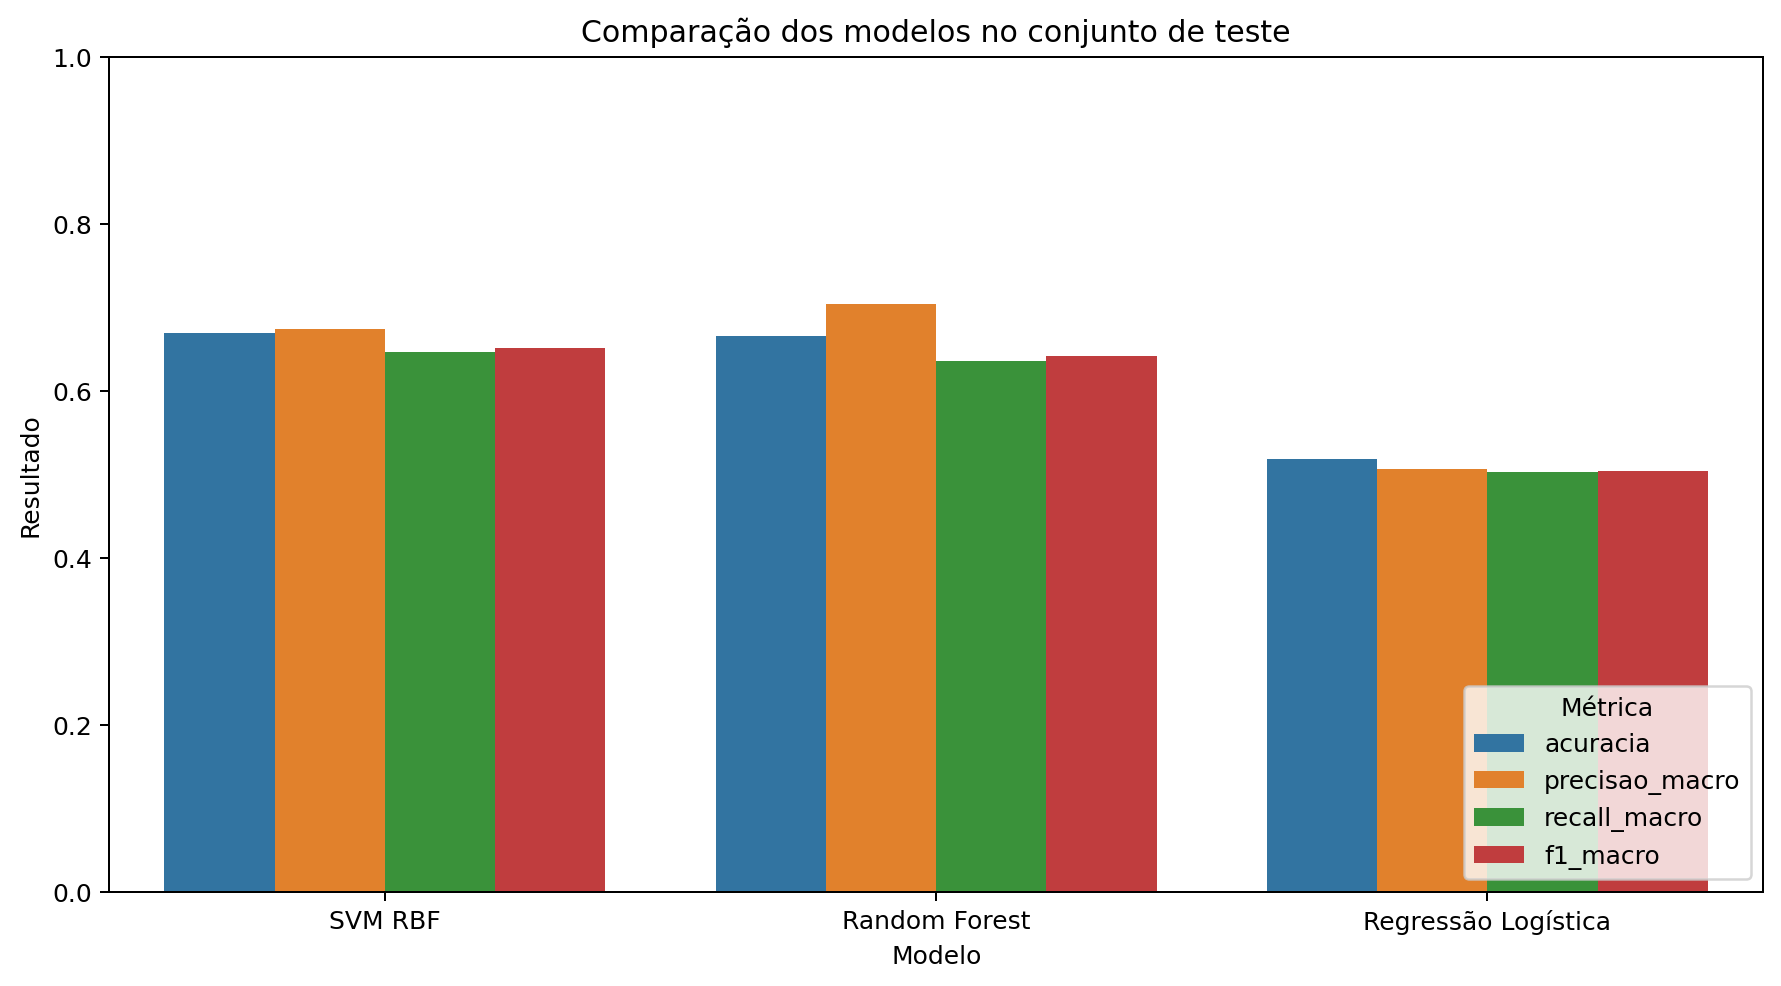
\includegraphics[width=0.9\textwidth]{images/05_comparacao_modelos.png}
\caption{Comparação entre as métricas dos modelos avaliados.}
\label{fig:modelos}
\end{figure}

\subsection{Resultados por classe}

A Tabela~\ref{tab:classesresultado} mostra o relatório da SVM. Papel, papelão, plástico e metal apresentaram F1 próximo ou superior a 68\%. Rejeito teve precisão de 69,70\%, mas recall de somente 36,51\%, indicando que o modelo foi conservador ao atribuir essa classe e deixou de reconhecer grande parte dos rejeitos reais.

\begin{table}[H]
\centering
\caption{Métricas por classe para a SVM RBF}
\label{tab:classesresultado}
\begin{tabular}{lrrrr}
\toprule
\textbf{Classe} & \textbf{Precisão} & \textbf{Recall} & \textbf{F1} & \textbf{Amostras} \\
\midrule
Metal & 67,35\% & 68,75\% & 68,04\% & 240 \\
Papel & 68,28\% & 70,78\% & 69,51\% & 219 \\
Papelão & 67,96\% & 71,10\% & 69,49\% & 173 \\
Plástico & 64,67\% & 72,95\% & 68,56\% & 281 \\
Rejeito & 69,70\% & 36,51\% & 47,92\% & 126 \\
Vidro & 66,31\% & 67,39\% & 66,85\% & 184 \\
\bottomrule
\end{tabular}
\end{table}

Na matriz de confusão, os principais erros envolveram plástico confundido com metal ou vidro, papel confundido com papelão e rejeito confundido com plástico ou metal. Esses resultados são coerentes com as semelhanças visuais entre embalagens transparentes, superfícies metálicas e materiais deformados.

\begin{figure}[H]
\centering
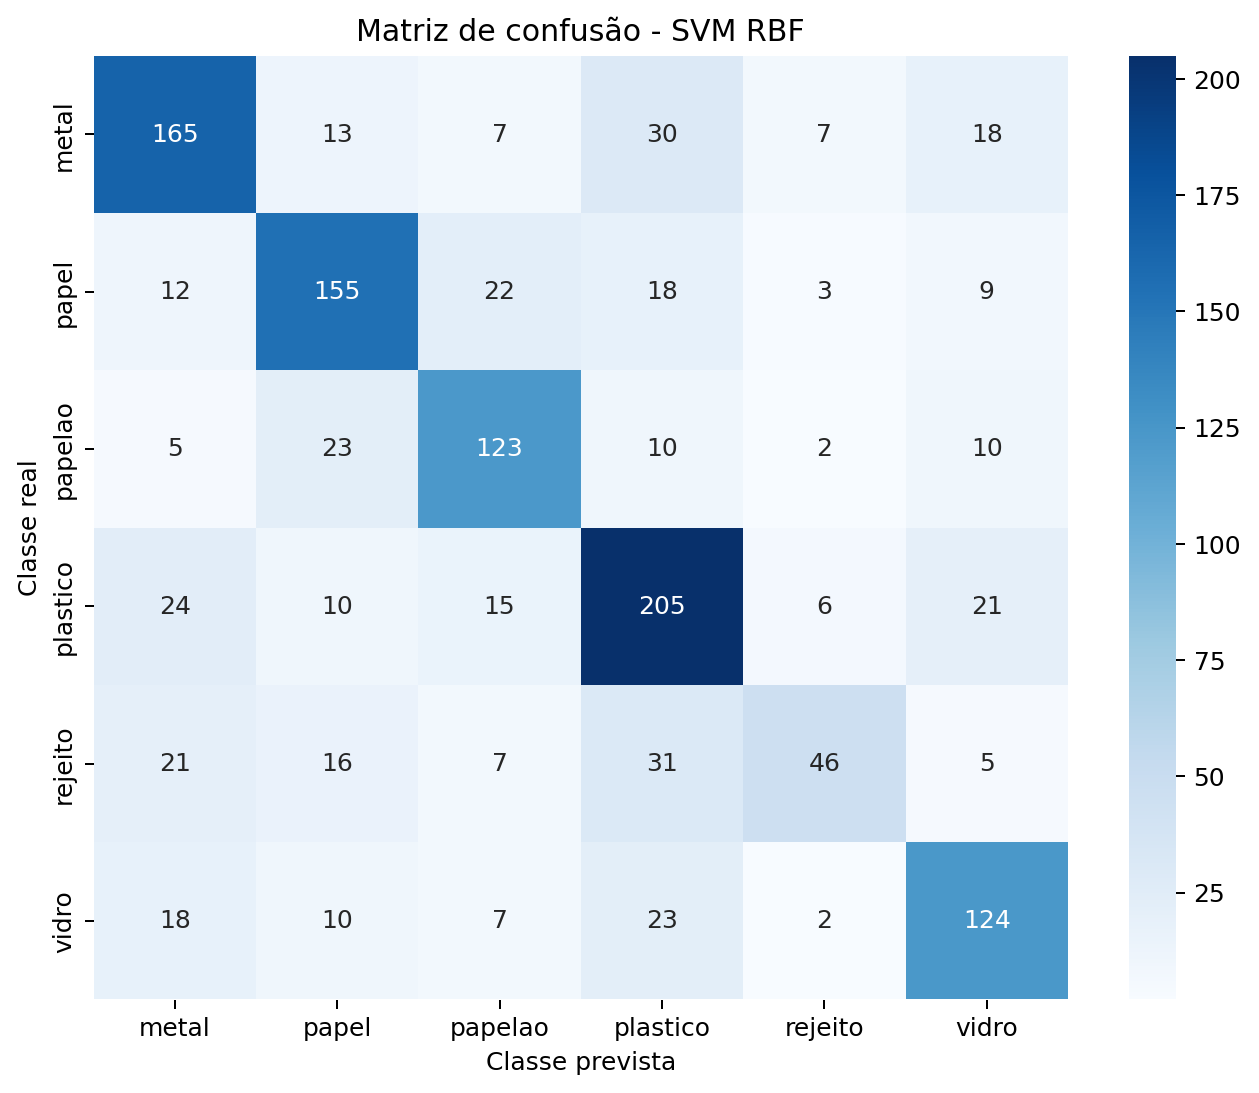
\includegraphics[width=0.79\textwidth]{images/matriz_confusao_svm_rbf.png}
\caption{Matriz de confusão da SVM RBF no conjunto de teste.}
\label{fig:matriz}
\end{figure}

\subsection{Generalização entre bases}

O experimento de mudança de domínio apresentou a evidência mais relevante do trabalho. Quando treinada somente com imagens da TrashNet, a SVM atingiu acurácia de 68,77\% e F1 macro de 67,49\% no teste interno. Quando o mesmo modelo foi aplicado à RealWaste, a acurácia caiu para 24,62\% e o F1 macro para 17,21\%.

\begin{table}[H]
\centering
\caption{Desempenho do modelo treinado somente na TrashNet}
\label{tab:dominio}
\begin{tabular}{lrrrr}
\toprule
\textbf{Cenário} & \textbf{Acurácia} & \textbf{Precisão macro} & \textbf{Recall macro} & \textbf{F1 macro} \\
\midrule
Teste interno TrashNet & 68,77\% & 71,62\% & 65,69\% & 67,49\% \\
Teste externo RealWaste & 24,62\% & 18,97\% & 19,51\% & 17,21\% \\
\bottomrule
\end{tabular}
\end{table}

\begin{figure}[H]
\centering
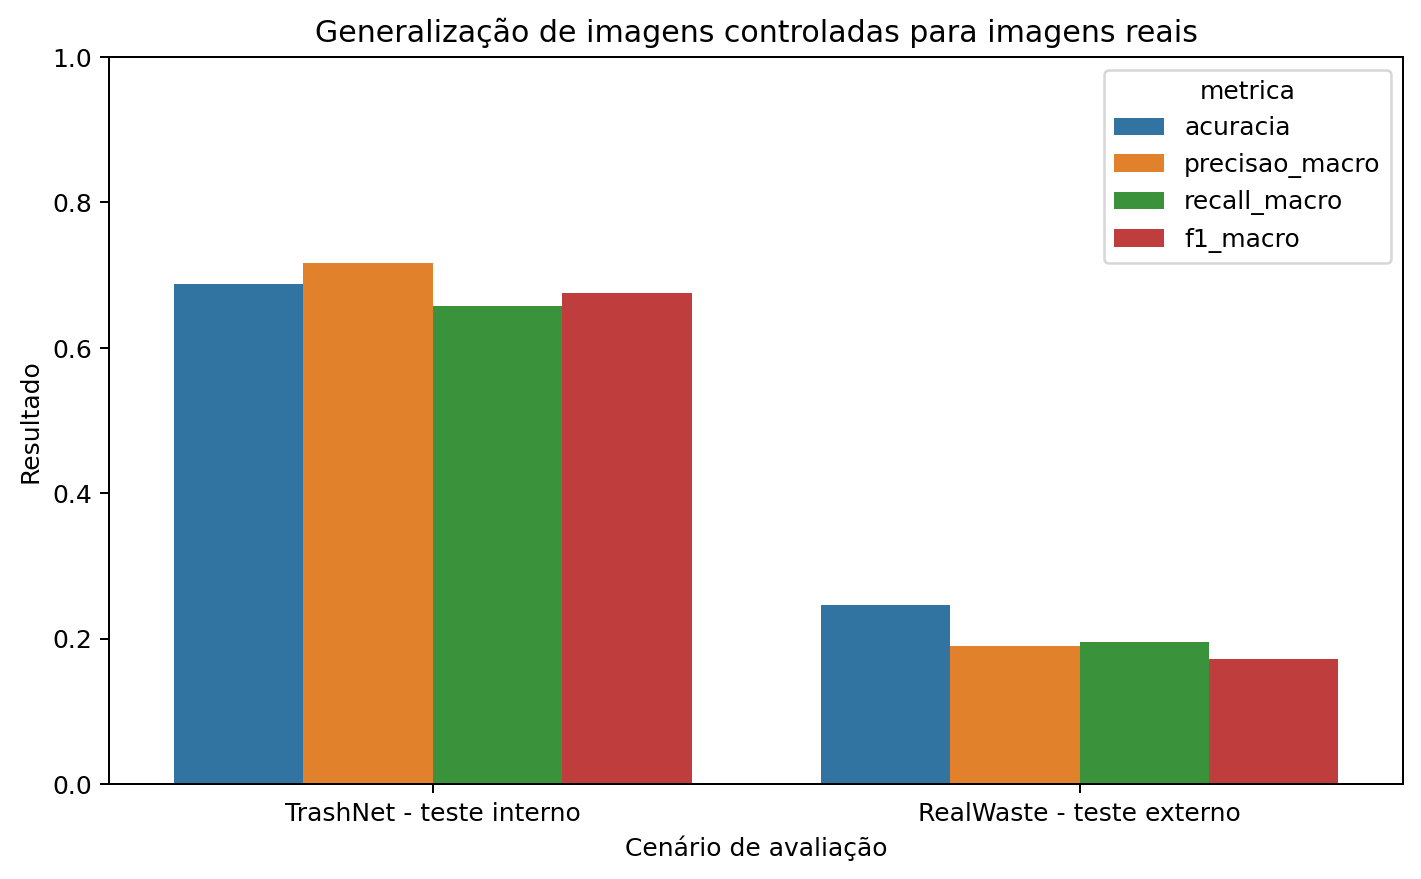
\includegraphics[width=0.86\textwidth]{images/06_mudanca_dominio.png}
\caption{Queda de desempenho ao transferir o modelo de imagens controladas para imagens reais.}
\label{fig:dominio}
\end{figure}

A hipótese de perda de desempenho fora do ambiente controlado foi confirmada. A diferença mostra que o modelo aprendeu características específicas da TrashNet, como fundo claro, iluminação e enquadramento, que não se mantêm na RealWaste. O treinamento combinado aumentou o F1 macro no teste geral para 65,06\%, reforçando a necessidade de utilizar amostras representativas do ambiente de aplicação.

\section{Implantação experimental e valor gerado}

O melhor modelo foi salvo em formato Joblib e integrado a uma API desenvolvida com FastAPI. O endpoint de consulta recebe um arquivo de imagem, aplica o mesmo pré-processamento do treinamento e devolve a classe prevista, o nome do modelo e uma confiança aproximada calculada a partir das pontuações da SVM. A API é opcional e deve ser considerada um protótipo, não um sistema de decisão automática.

Em uma aplicação futura, os registros da API poderão apoiar a identificação das classes mais consultadas, o acompanhamento de erros e a seleção de novas imagens para retreinamento. Para uma organização, essas informações podem orientar campanhas de descarte, treinamento de equipes e ajustes na distribuição dos coletores. Tais decisões exigem dados reais de uso; a quantidade de imagens em um dataset não representa a frequência de resíduos produzidos por uma empresa ou cidade.

O código, as instruções de reprodução e os resultados estão organizados no repositório \url{https://github.com/leobonatto/Planterra2.0}, na pasta \texttt{EcoScan}. Os arquivos brutos das bases não são versionados devido ao tamanho; os endereços oficiais e o procedimento de obtenção estão documentados no projeto.

\section{Limitações e trabalhos futuros}

A primeira limitação é a representação das imagens por atributos manuais. HOG e histogramas de cor são adequados para comparar modelos tradicionais, mas não capturam toda a complexidade visual dos resíduos. Redes neurais convolucionais e transferência de aprendizado podem melhorar os resultados em trabalhos futuros.

A segunda limitação é a origem dos dados. A RealWaste foi coletada em uma instalação australiana e pode não representar resíduos, embalagens e condições de captura encontradas no Brasil. Além disso, cada imagem possui um único rótulo, mesmo quando há materiais misturados. Não existem informações de peso, volume, data, custo de triagem ou destino final.

O experimento utilizou uma divisão estratificada fixa, e os resultados podem variar com outras amostras. Uma avaliação futura deve empregar validação cruzada, ajuste sistemático de hiperparâmetros e um conjunto externo brasileiro. Também devem ser realizados testes com usuários para verificar se a ferramenta reduz o tempo de triagem e se suas sugestões são compreendidas corretamente.

\section{Conclusão}

O projeto aplicou o ciclo completo de Mineração de Dados a 6.114 imagens das bases TrashNet e RealWaste. O fluxo incluiu compreensão do problema, validação e padronização dos dados, análise exploratória, transformação das imagens, tratamento do desbalanceamento, comparação de modelos, avaliação e implantação experimental.

A SVM RBF apresentou o melhor F1 macro, com 65,06\%, enquanto o Random Forest obteve resultado próximo e custo de treinamento muito menor. O desempenho por classe mostrou que rejeito foi a categoria mais difícil, principalmente pelo baixo recall. A avaliação externa confirmou que um modelo treinado em fotografias controladas não se transfere automaticamente para imagens reais: o F1 macro caiu de 67,49\% para 17,21\%.

Os resultados respondem à pergunta principal e confirmam que a qualidade não depende apenas da quantidade de imagens, mas da semelhança entre os dados de treinamento e o ambiente real. O EcoScan continua sendo uma proposta viável como ferramenta de apoio, desde que receba imagens representativas do contexto de uso, seja monitorado por métricas por classe e mantenha supervisão humana nas previsões incertas.

\begin{thebibliography}{99}
\bibitem{wirth2000crisp} WIRTH, R.; HIPP, J. CRISP-DM: Towards a standard process model for data mining. In: \textit{Proceedings of the 4th International Conference on the Practical Applications of Knowledge Discovery and Data Mining}. 2000. p. 29--39.
\bibitem{single2023realwaste} SINGLE, S.; IRANMANESH, S.; RAAD, R. RealWaste: A novel real-life data set for landfill waste classification using deep learning. \textit{Information}, v. 14, n. 12, p. 633, 2023. DOI: \url{https://doi.org/10.3390/info14120633}.
\bibitem{thung2016trashnet} THUNG, G.; YANG, M. TrashNet: Dataset of images of trash. 2016. Disponível em: \url{https://github.com/garythung/trashnet}. Acesso em: 13 nov. 2026.
\bibitem{dalal2005hog} DALAL, N.; TRIGGS, B. Histograms of oriented gradients for human detection. In: \textit{IEEE Computer Society Conference on Computer Vision and Pattern Recognition}. 2005. p. 886--893. DOI: \url{https://doi.org/10.1109/CVPR.2005.177}.
\bibitem{pedregosa2011scikit} PEDREGOSA, F. et al. Scikit-learn: Machine learning in Python. \textit{Journal of Machine Learning Research}, v. 12, p. 2825--2830, 2011.
\bibitem{harris2020numpy} HARRIS, C. R. et al. Array programming with NumPy. \textit{Nature}, v. 585, p. 357--362, 2020. DOI: \url{https://doi.org/10.1038/s41586-020-2649-2}.
\bibitem{mckinney2010pandas} MCKINNEY, W. Data structures for statistical computing in Python. In: \textit{Proceedings of the 9th Python in Science Conference}. 2010. p. 56--61.
\bibitem{hunter2007matplotlib} HUNTER, J. D. Matplotlib: A 2D graphics environment. \textit{Computing in Science \& Engineering}, v. 9, n. 3, p. 90--95, 2007. DOI: \url{https://doi.org/10.1109/MCSE.2007.55}.
\bibitem{waskom2021seaborn} WASKOM, M. L. Seaborn: Statistical data visualization. \textit{Journal of Open Source Software}, v. 6, n. 60, p. 3021, 2021. DOI: \url{https://doi.org/10.21105/joss.03021}.
\end{thebibliography}

\end{document}
